
%(BEGIN_QUESTION)
% Copyright 2007, Tony R. Kuphaldt, released under the Creative Commons Attribution License (v 1.0)
% This means you may do almost anything with this work of mine, so long as you give me proper credit

Calculate the amount of pressure applied to each side of the differential pressure transmitter (in units of PSI) when there is 9 feet of liquid level in the process vessel.  Note the pressure gauge at the top of the vessel registering the amount of vapor pressure inside:

$$\includegraphics[width=15.5cm]{i02950x01.eps}$$

\vskip 10pt

$P_{high}$ = \underbar{\hskip 50pt} PSIG \hskip 100pt $P_{low}$ = \underbar{\hskip 50pt} PSIG

\vskip 10pt

Also, calculate the {\it differential} pressure seen by the transmitter (in units of PSI):

\vskip 10pt

$\Delta P$ = \underbar{\hskip 50pt} PSID

\vskip 10pt

\underbar{file i02950}
%(END_QUESTION)





%(BEGIN_ANSWER)

$P_{high}$ = {\bf 72.487} PSIG \hskip 100pt $P_{low}$ = {\bf 68} PSIG

\vskip 10pt

$\Delta P$ = {\bf 4.487} PSID

%(END_ANSWER)





%(BEGIN_NOTES)

%INDEX% Measurement, level: hydrostatic pressure + vapor pressure compensation

%(END_NOTES)


